\subsubsection{Which implementation technologies and tools are adopted by software development professionals?}
\label{tools}
\anindya{Implementation or development??}
Our survey included five questions to find technologies and tools that are adopted by software development professionals. To answer this question fully, we report the following results:

\begin{itemize}
\item Technology Platform (Q 9).
\item Operating System (Q 10).
\item Programming Language (Q 11).
\item Framework (Q 12).
\item IDE (Q 13).
\end{itemize}


\paragraph{Technology Platforms}
Participants were allowed to choose multiple options. As shown in Figure \ref{fig:platforms}, most of our survey respondents (80\%) work for the web platform. The rests are mobile (45\%), desktop (30\%)\anindya{is it the best name?}\khalid{It was one of the choices of this closed question}, embedded/IoT (8\%). Interestingly, from the 2020 survey of JetBrains \cite{JetBrains2020}, we have observed quite a similar result. The survey shows that websites are the most common type of application developers work on, and the web platform is the most preferable and popular to develop, followed by desktop and mobile. This result shows that clients of software products heavily prefer or need web-based services. We have conducted a cross-aspect analysis to identify any relationship between the technology platform and the requirement gathering process. The bubble charts in Figure \ref{fig:requirement technology cross analysis} visualize the cross-aspect analysis. It is clear from the figure that the requirement gathering process is mostly practiced in GUI-based development (e.g., web, desktop, mobile).
\begin{figure}[h]
\centering
  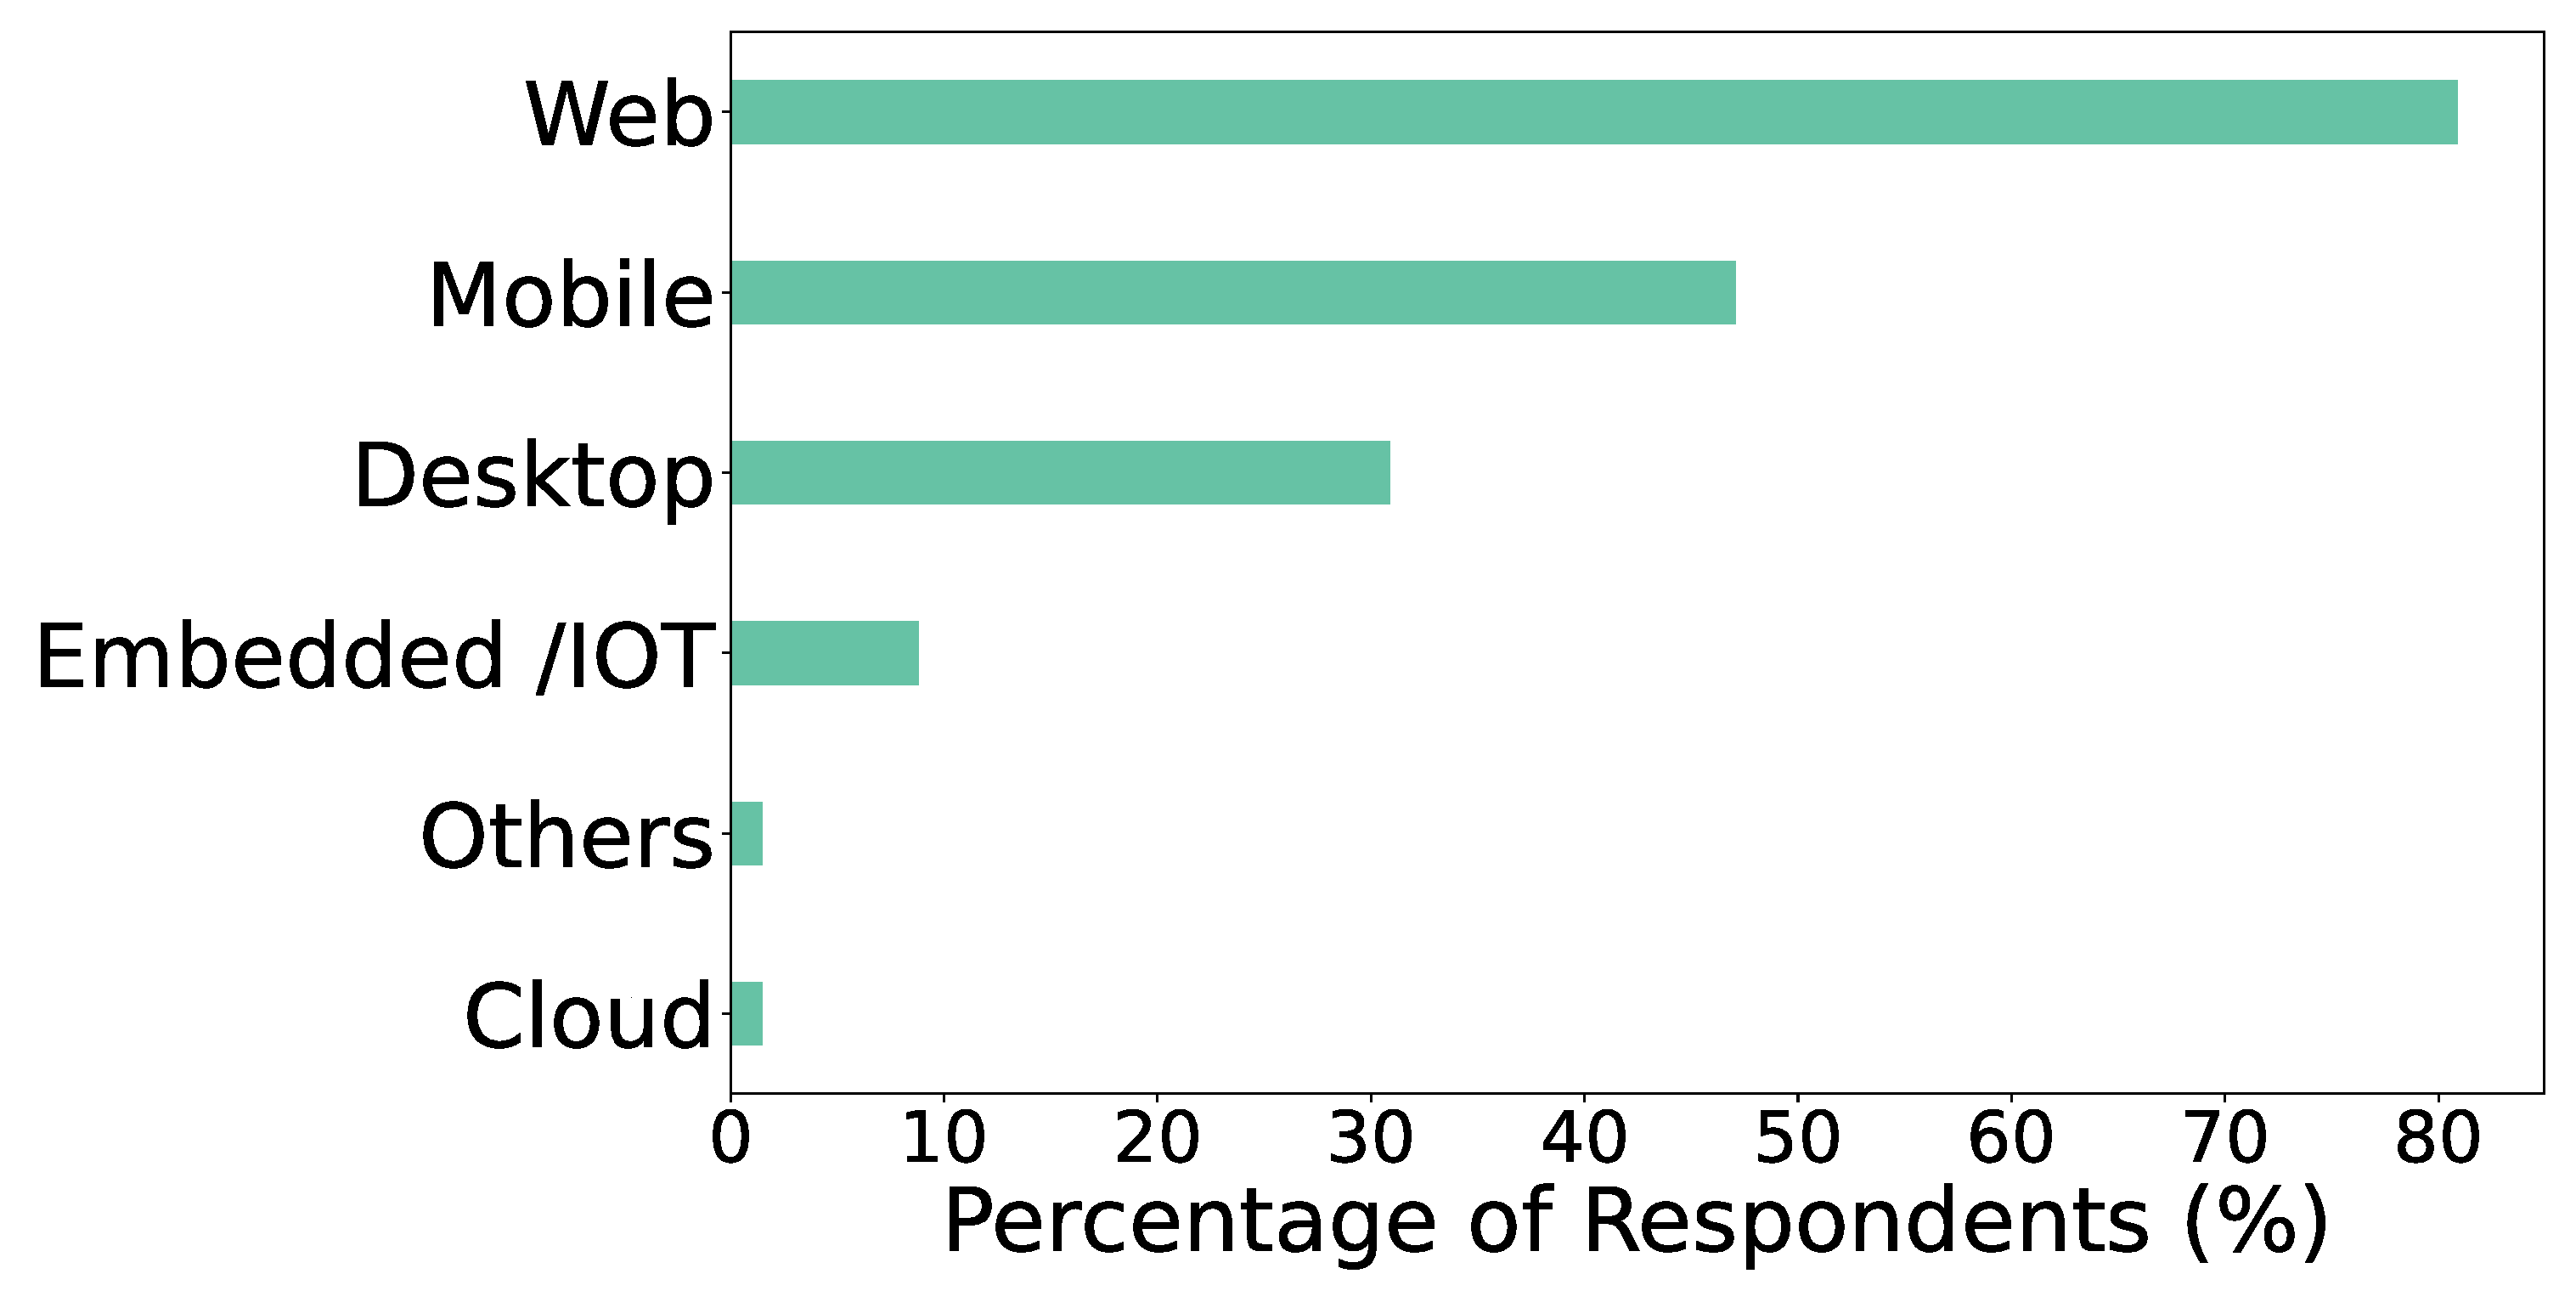
\includegraphics[scale=0.18]{Figures/Respondents_Technologies}
  \caption{Technology Platforms}
  \label{fig:platforms}
\end{figure}

\begin{figure}[h]
\centering
  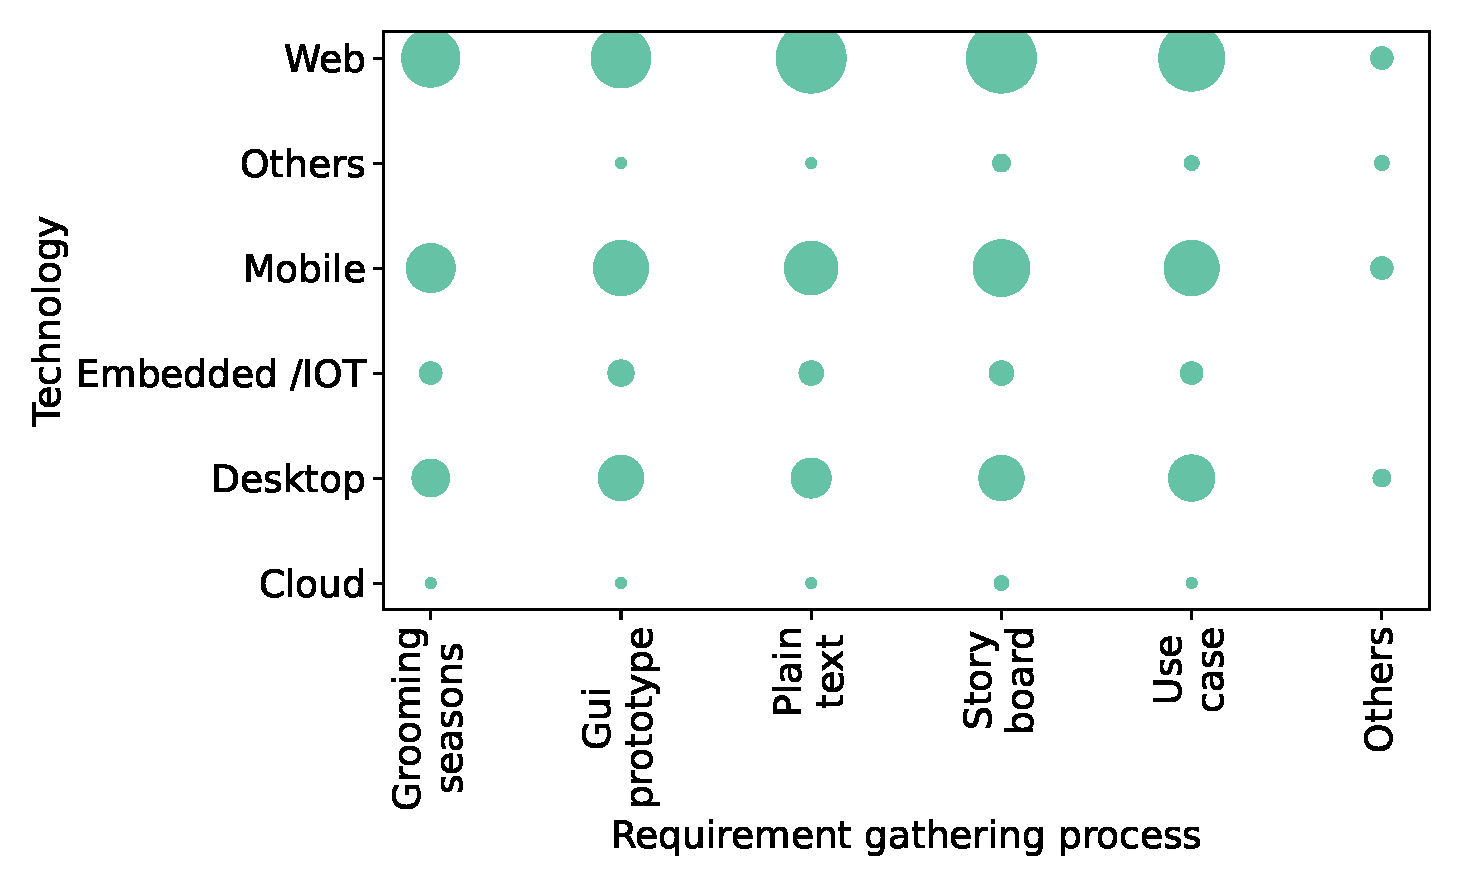
\includegraphics[scale=0.47]{Figures/Requirement_Technology_Cross_Analysis.eps}
  \caption{Cross aspect analysis of requirement gathering process and technology platform}
  \label{fig:requirement technology cross analysis}
\end{figure}

\boxtext{Web based software services top the list of development technologies.}


\paragraph{Operating Systems}
In our survey, as per Figure \ref{fig:os}, we have found that most of our respondents replied that they use Linux based operating system (56\%) as a primary operating system for their development. The second frequently used operating system is Windows (45\%), and 28\% of the respondents use macOS. We observed similar scenarios in the 2018 and 2019 StackOverflow (SO) surveys \cite{StackoverflowSurvey2018,StackoverflowSurvey2019}. However, Windows ranked first in the 2020 survey of both SO and JetBrains \cite{StackoverflowSurvey2020, JetBrains2020}. The game-changing phenomenon may be related to the newly included WSL (Windows Subsystem for Linux). This feature allows users to perform almost any Linux-specific task on Windows. We anticipated that the use of OS might be related to professional experience. Among the participants, senior/expert developers have higher rates of Linux usage. This suggests that senior/expert developers may prefer Linux over other operating systems. \anindya{The last line is not clear.}\partha{rephrased}. We have conducted the Mann Whitney U test and our anticipation was found correct ($p=0.024$). %Senior developers prefer Linux over other operating systems.

\begin{figure}[h]
\centering
  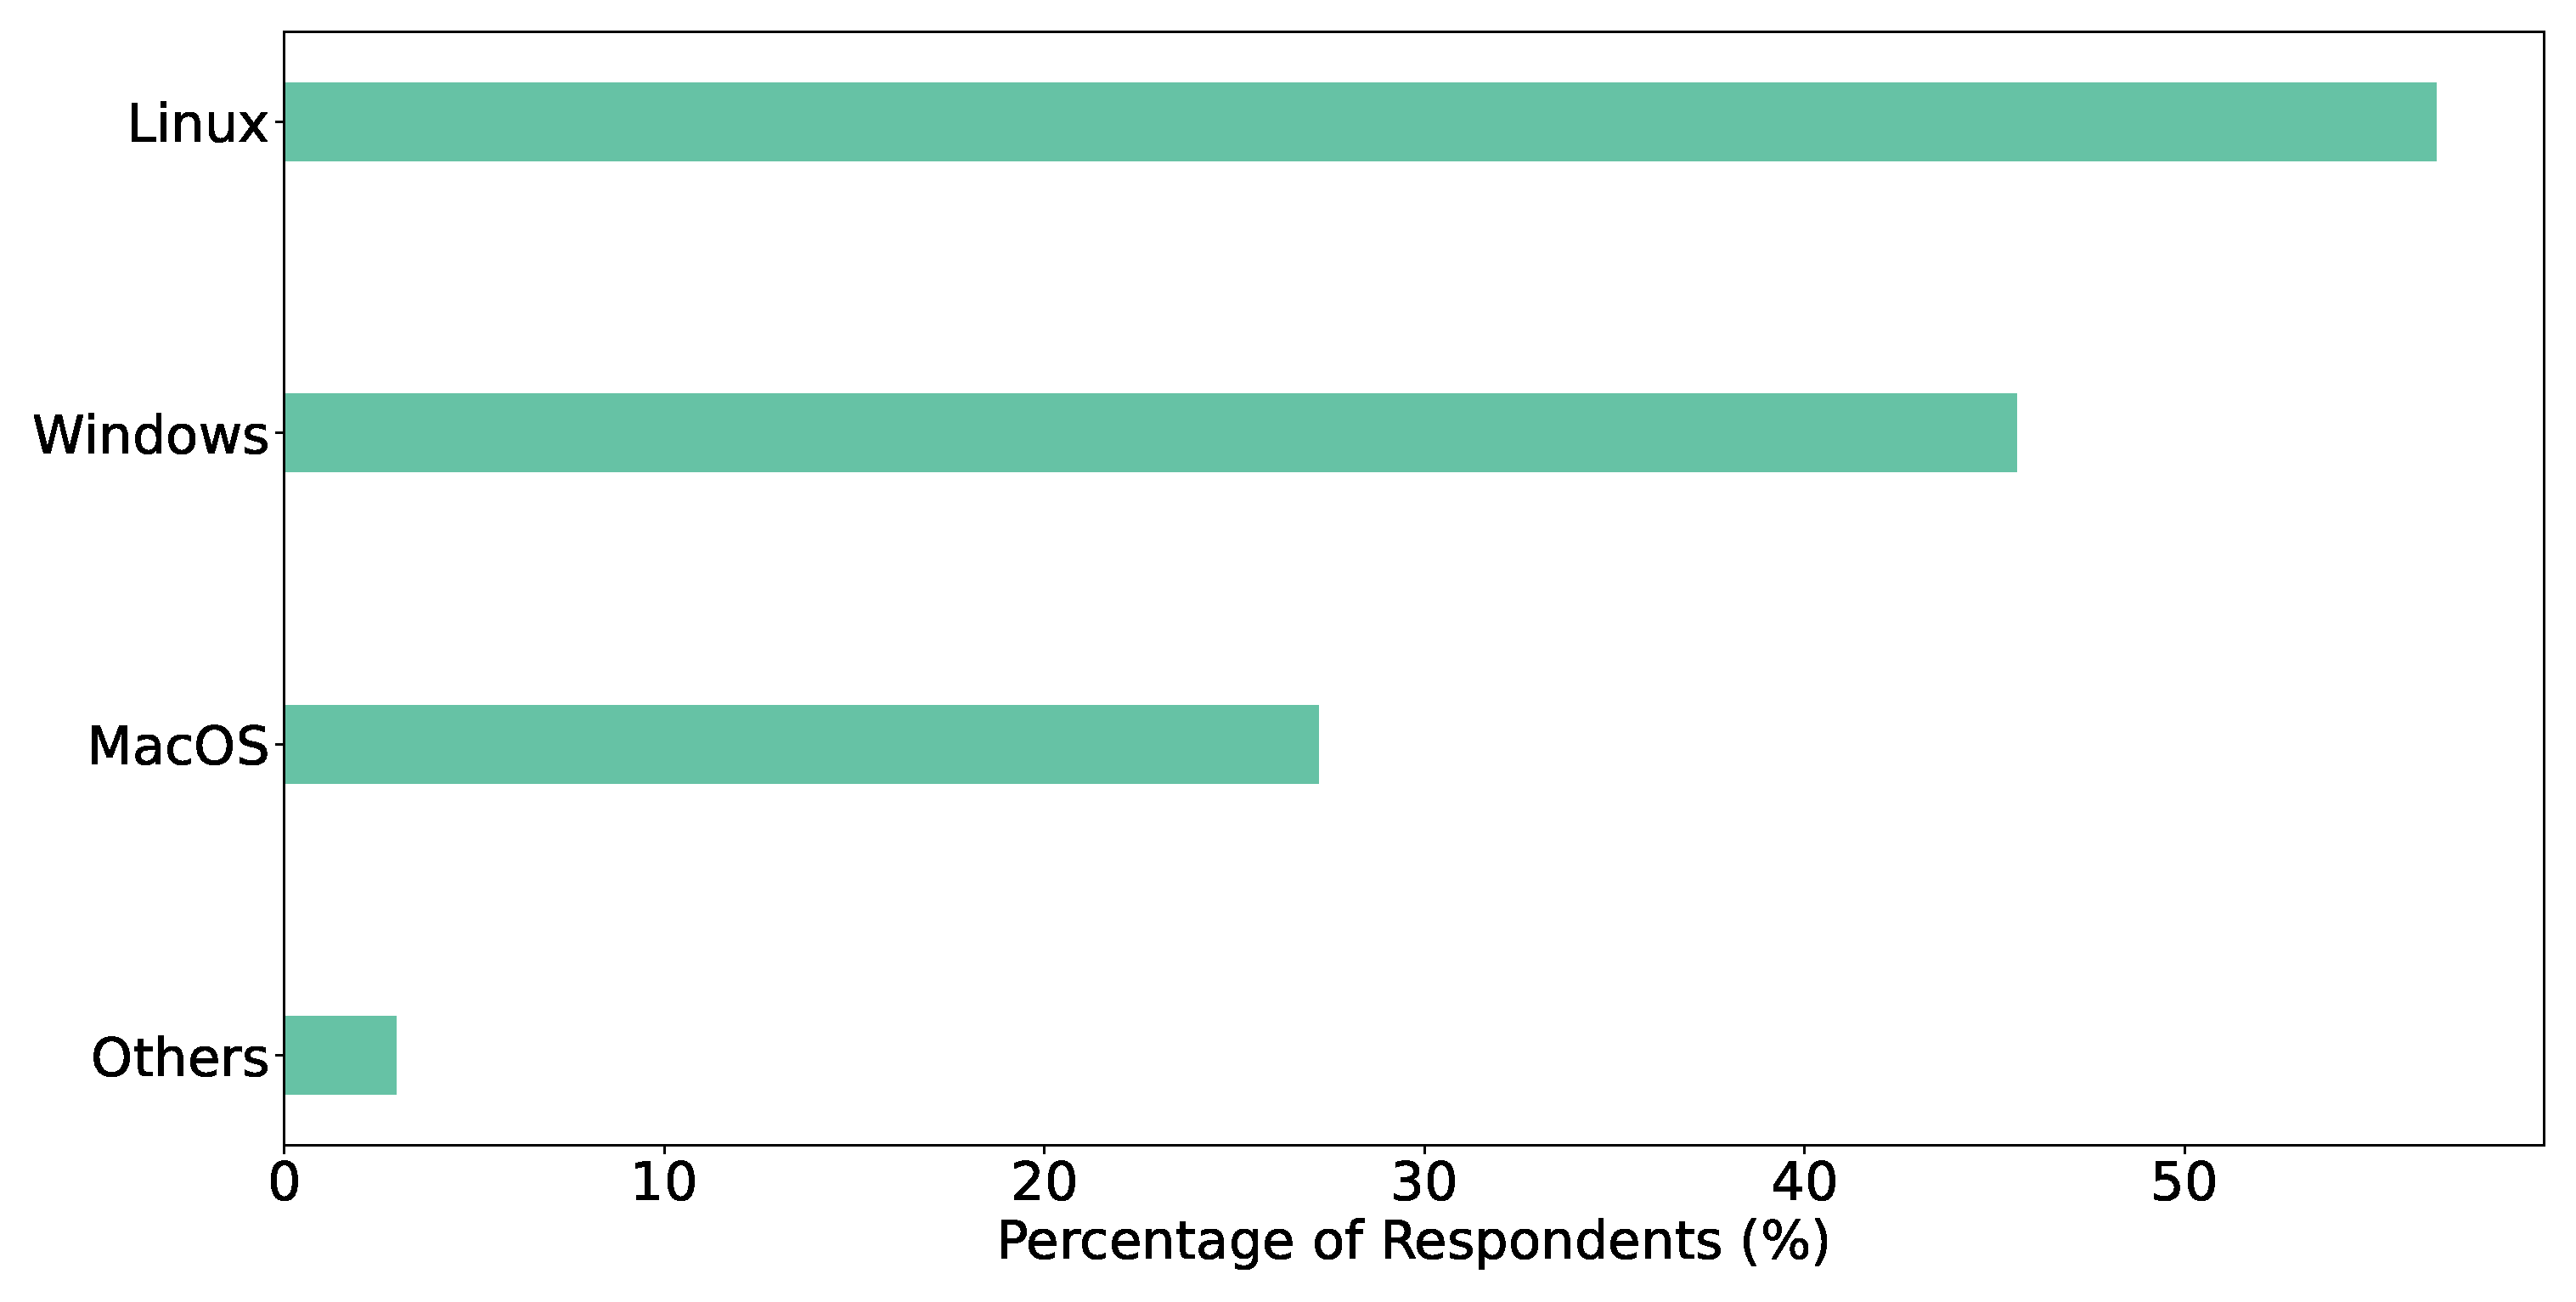
\includegraphics[scale=0.17]{Figures/Respondents_os}
  \caption{Operating Systems}
  \label{fig:os}
\end{figure}


\paragraph{Programming Languages}
According to Figure \ref{fig:languages}, around 65\% and 60\% of our respondents use JavaScript and Java, respectively, which are the two most used languages in Bangladesh. This result seems expected as both JavaScript and Java are popular for web and mobile platforms, and a great percentage of our survey participants develop for both web and mobile platforms, as discussed earlier in this section. Other languages like PHP (25\%), Python (25\%), and C\# (18\%) are also used, which indicates that the software engineers are not biased towards a single specific language. Our survey result matches with the last two years' Stack Overflow survey and the GitHub stat. In all of the cases, JavaScript is the most used language, followed by Java and Python \cite{StackoverflowSurvey2020, StackoverflowSurvey2019, GithubStat}. The choice of programming languages used for development can have an important influence on the testing practices of a software company. We observed that users using mobile and web platforms mostly use Java and Javascript as programming languages. However, this is not statistically significant ($p=0.1$). Though the use of the operating system is influenced by programming language (e.g., Swift and macOS), we have not found any relation between the choice of programming language and the operating system.


\begin{figure}[h]
\centering
  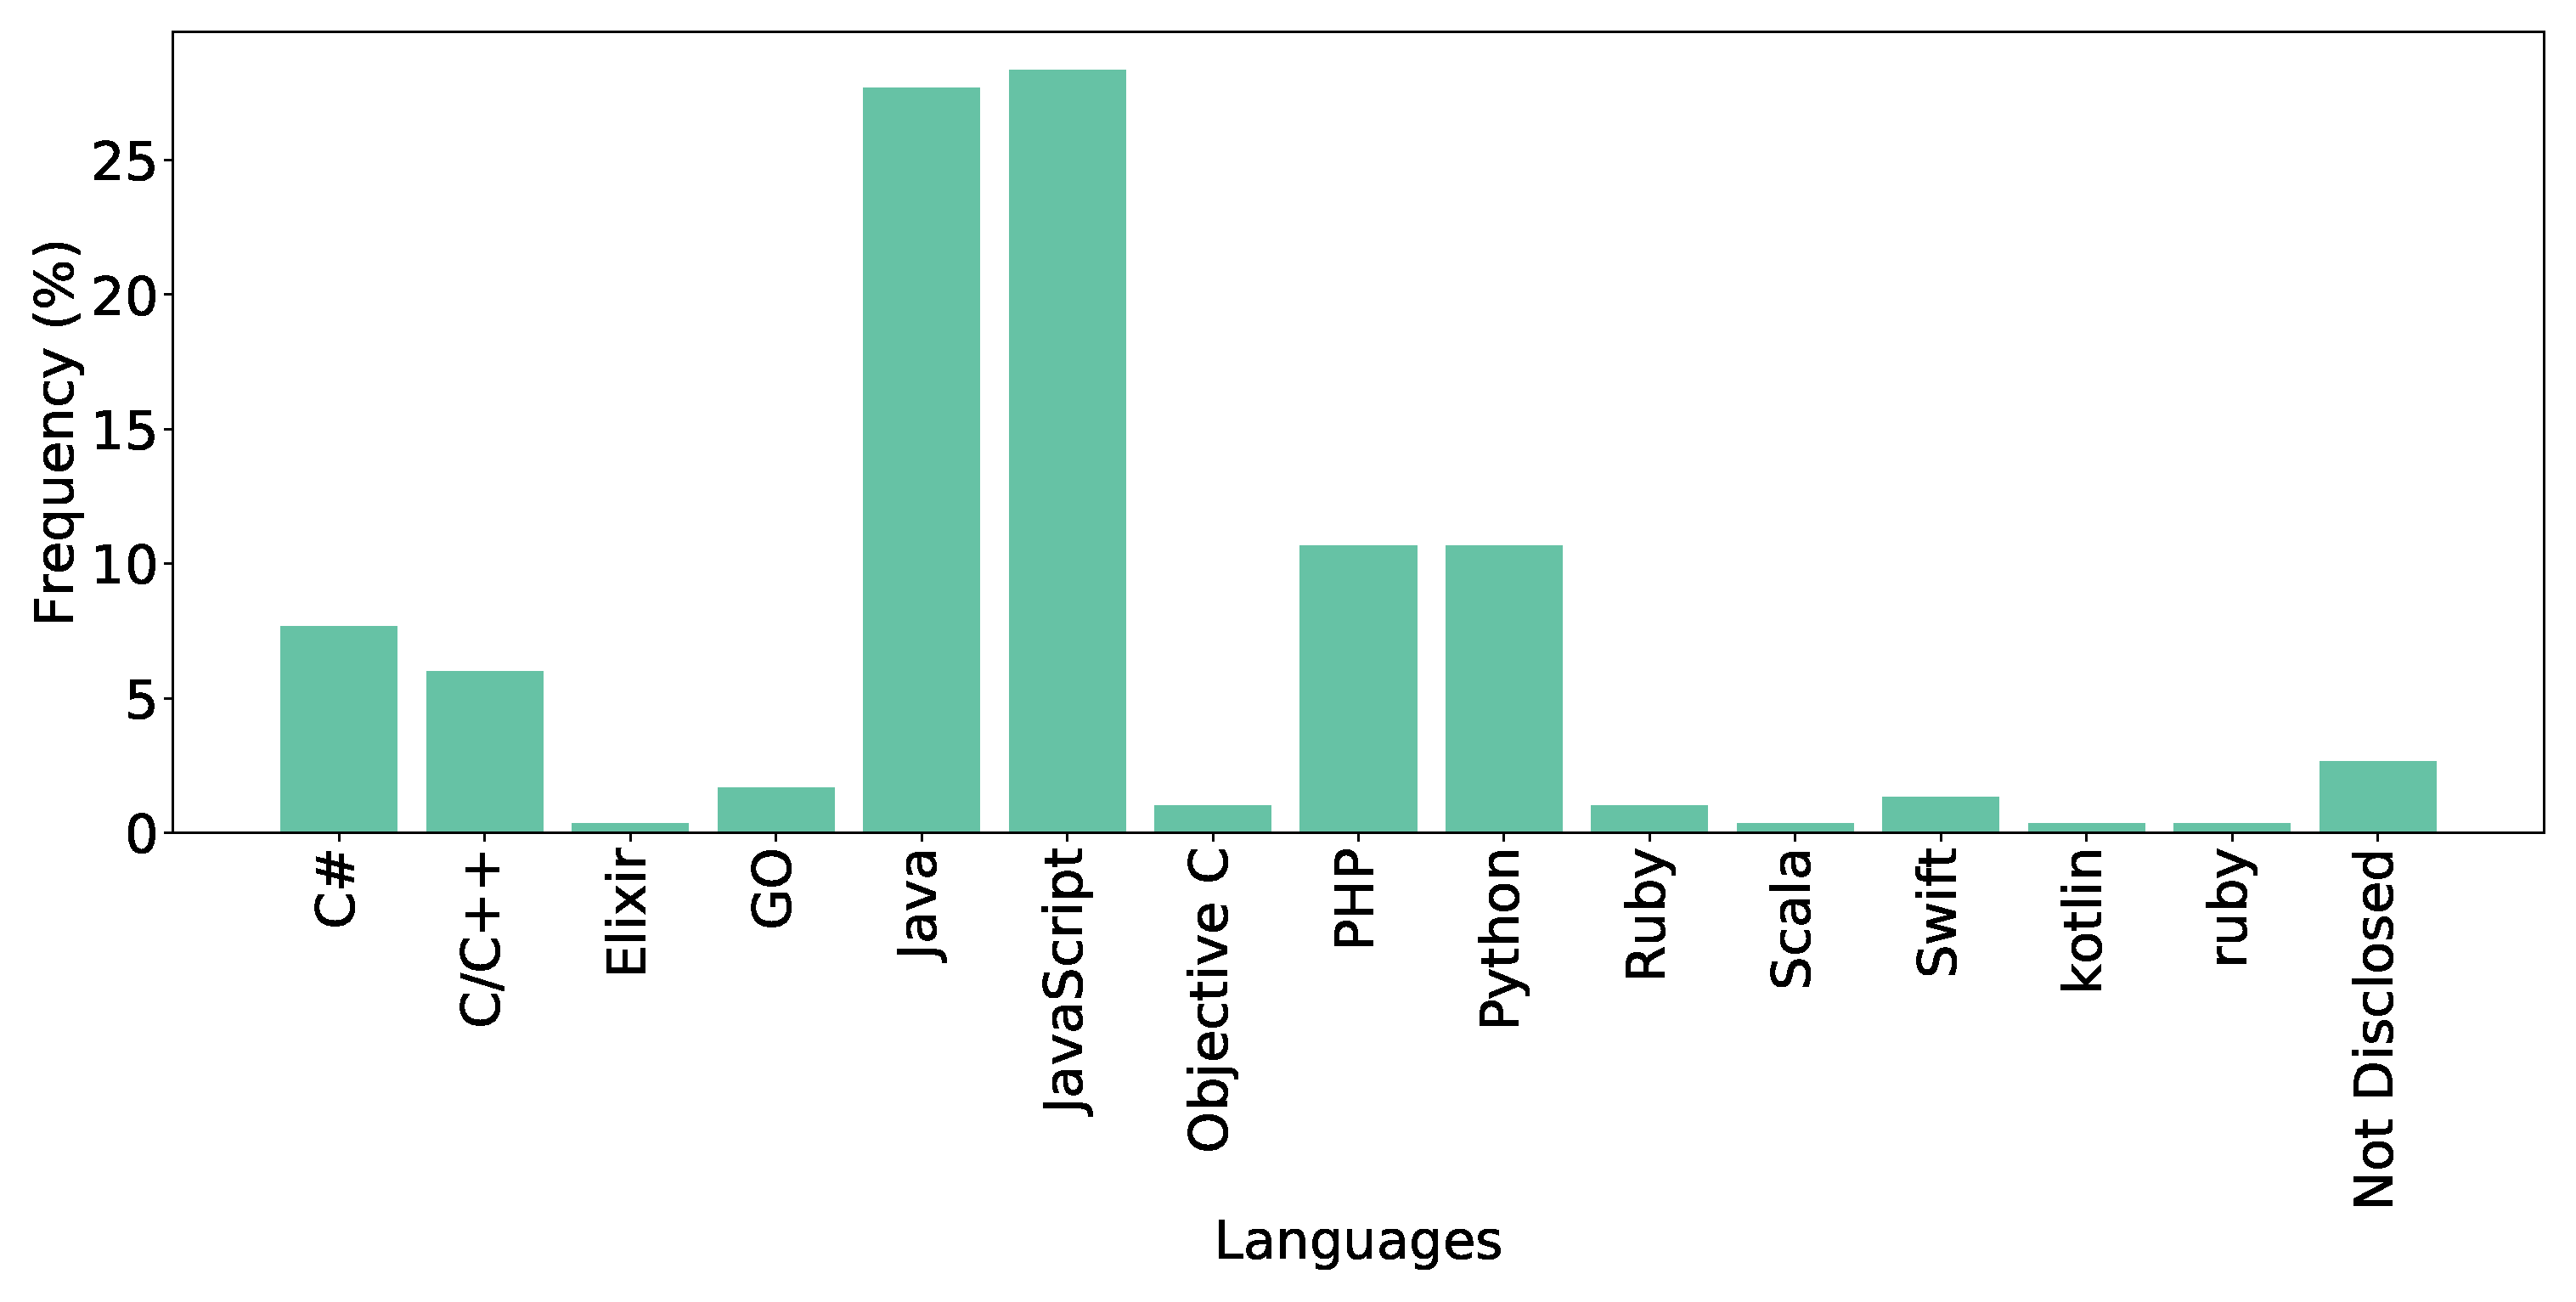
\includegraphics[scale=0.18]{Figures/Respondents_languages}
  \caption{Languages used in software development}
  \label{fig:languages}
\end{figure}

\paragraph{Frameworks used in development}
As shown in Figure \ref{fig:frameworks}, a variety of frameworks have been used during development. Spring boot (37\%) is the most used framework in the Bangladesh software industry, which is aligned with the result of Java's usage rate corresponding to Figure \ref{fig:languages}. Since JavaScript is the most used language of our respondents, they use various JavaScript frameworks such as React, Node.js, Angular, Express, etc., at an appreciable percentage. ASP.NET, Django, and Laravel are used in the same proportion based on around 15\% of our respondents. React, Swift, Ruby on Rails, Node.js, etc., are comparatively less used. Other than these, lots of frameworks such as Cocoa, Meteor, TestNG, Relay, Appium, CakePHP, etc., are also used in a comparatively small percentage. These are combinedly presented in the category named others. For web development, Django and Spring frameworks are mostly used in Bangladesh ($p=0.04$). We have compared our results with the Stack Overflow 2016 to 2020 survey\cite{StackoverflowSurvey2017, StackoverflowSurvey2018, StackoverflowSurvey2019, StackoverflowSurvey2020}. The only common framework in the top five list in both surveys is ASP.NET. In the stack overflow survey, we noticed that JavaScript-based frameworks (e.g., Jacqueline, Angular, React, Node.js) occupy the top positions (top five), which is not the case for our survey.

\begin{figure}[h]
\centering
  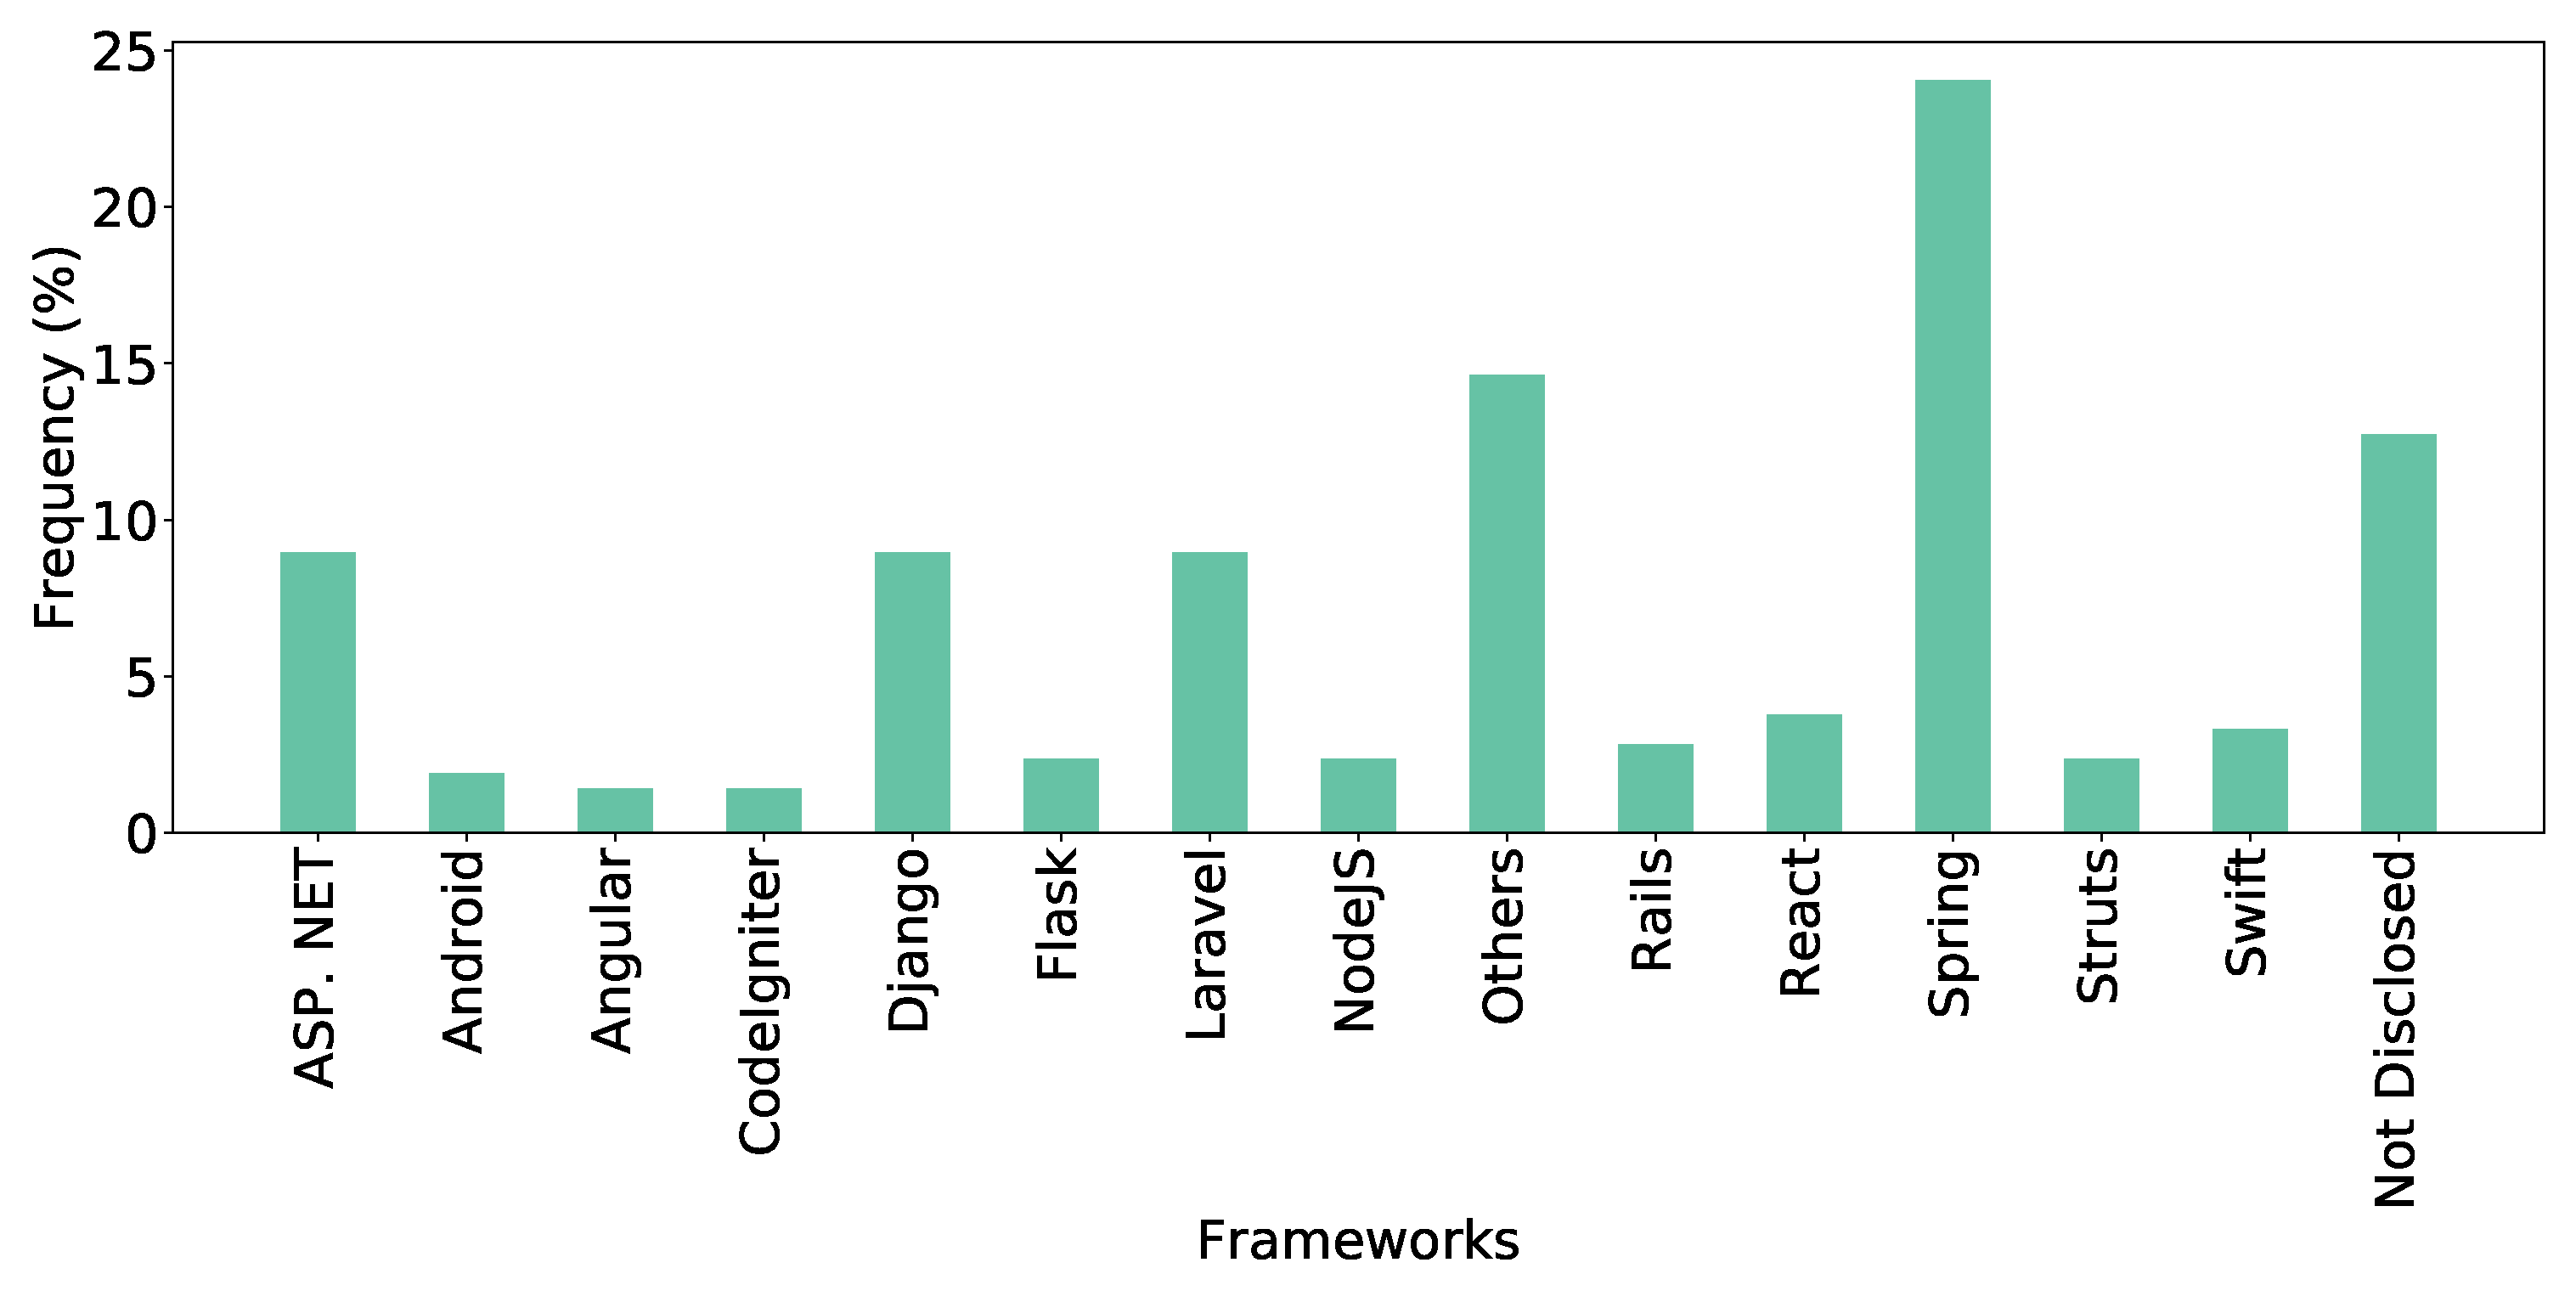
\includegraphics[scale=0.18]{Figures/Respondents_frameworks}
  \caption{Frameworks}
  \label{fig:frameworks}
\end{figure}

\paragraph{IDE's used by the respondent's}
According to Figure \ref{fig:IDEs}, IntelliJ, a Java integrated development tool for developing software for the enterprise, mobile, and web application, is used by most respondents (43\%). The other IDEs used in SE industries are Visual Studio (30\%), Eclipse (24\%), PyCharm (17\%), NetBeans (11\%), and Android Studio (7\%).

\begin{figure}[htbp]
\centering
  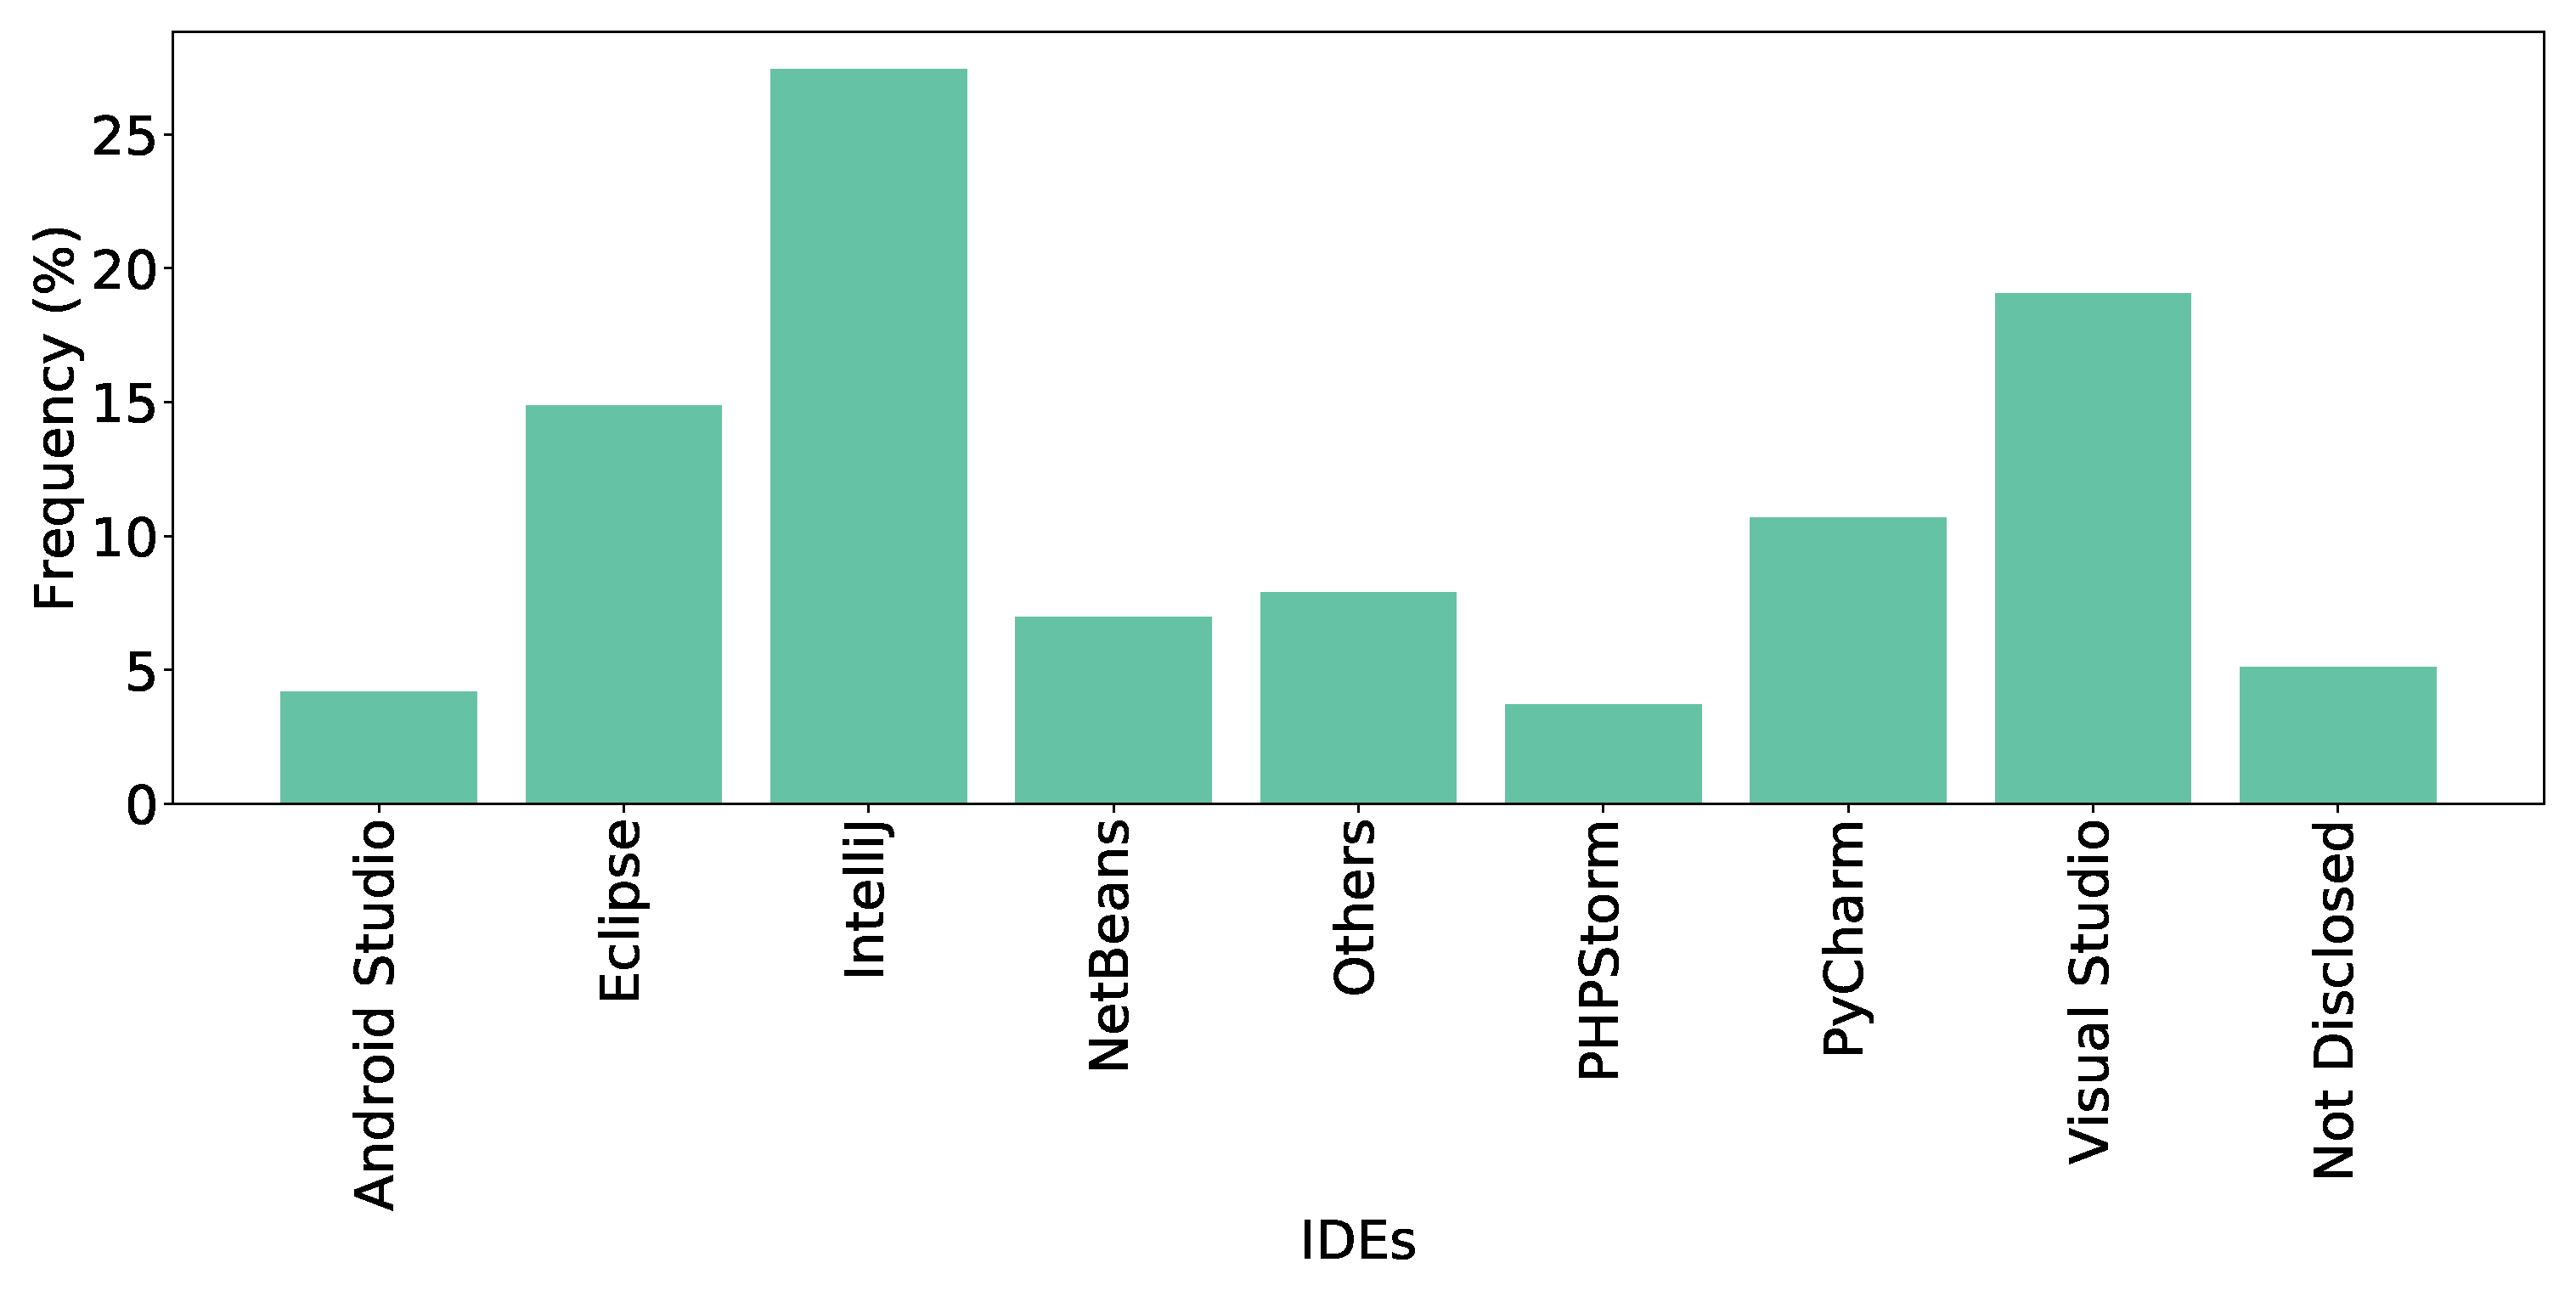
\includegraphics[scale=0.18]{Figures/Respondents_IDEs}
  \caption{IDE's}
  \label{fig:IDEs}
\end{figure}
